\section{R-trees}
\label{sec:rtree}
From \textcite{rtree}, an R-tree is a tree structure composed of nodes containing multi-dimensional data, facilitating range searches accross multiple dimensions. All data is stored as leaf nodes on the same level, which makes it a balanced tree. Each nodes is defined by a minimum bounding rectangle (MBR), which represent the range of the dimensions for that node and its child noeds. For leaf nodes the MBR represents the range of its data. A leaf node typically references data points rather than storing them directly in the tree. Figure \ref{fig:rtree} illustrates the node hierarchy within an R-tree, with the associated MBRs depicted in figure \ref{fig:mbrs}. An r-tree can be used to efficiently retrieve references to all data points within a certain range. This can drastically improves performance for queries in large datasets. When querying with an r-tree as a filter, only nodes with MBRs overlapping with the range of the query, potentially reducing the number of accessed nodes, and thereby also the number of accessed data points.

A typical application for r-trees is storing geospatial data, however the structure is not limited to that. For example it can be used for sorting people by age and last name.

\begin{figure}
    \centering
    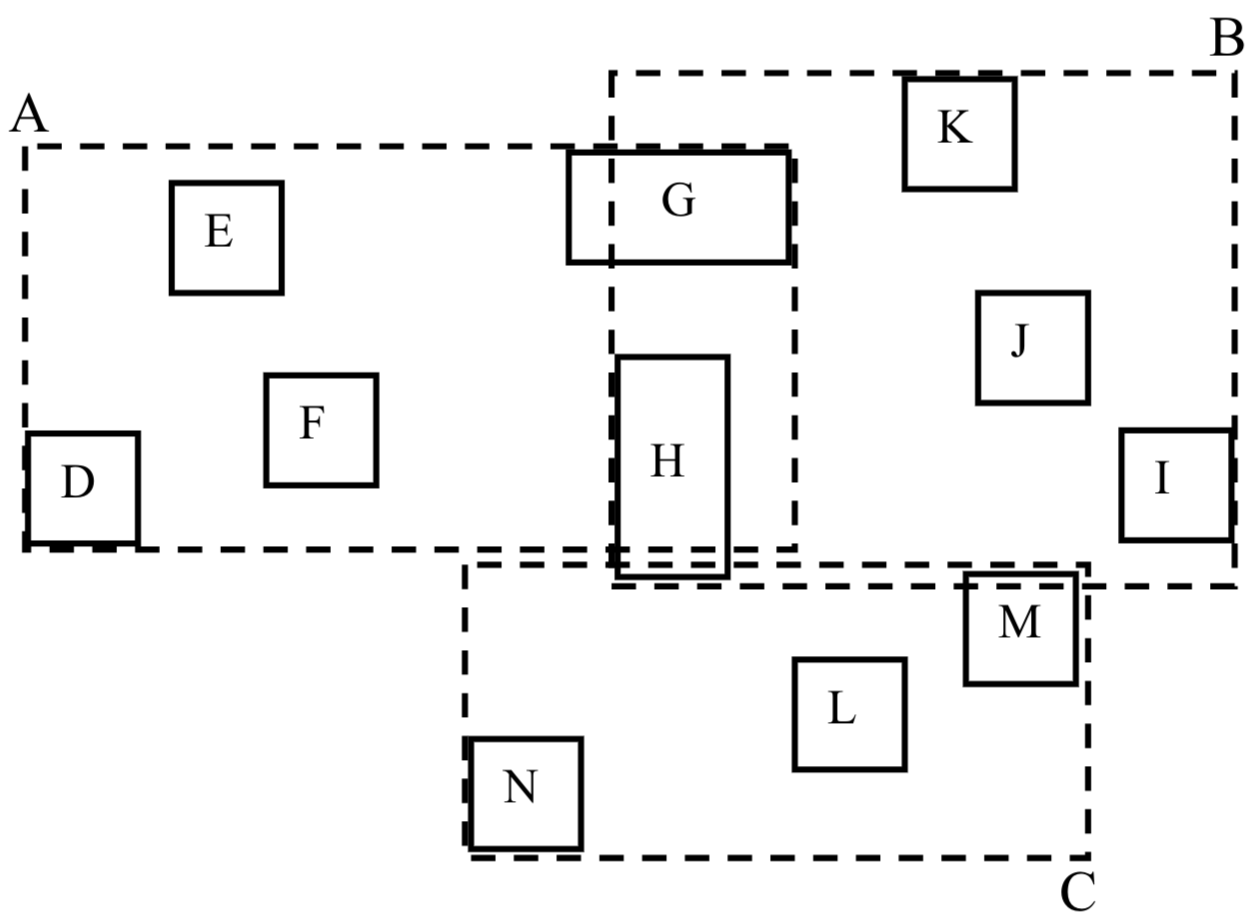
\includegraphics[width=0.5\linewidth]{./figures/mbrs.png}
    \caption{An example of data MBRs and their MBRs, from \cite{rtree}.}
    \label{fig:mbrs}
\end{figure}
\begin{figure}
    \centering
    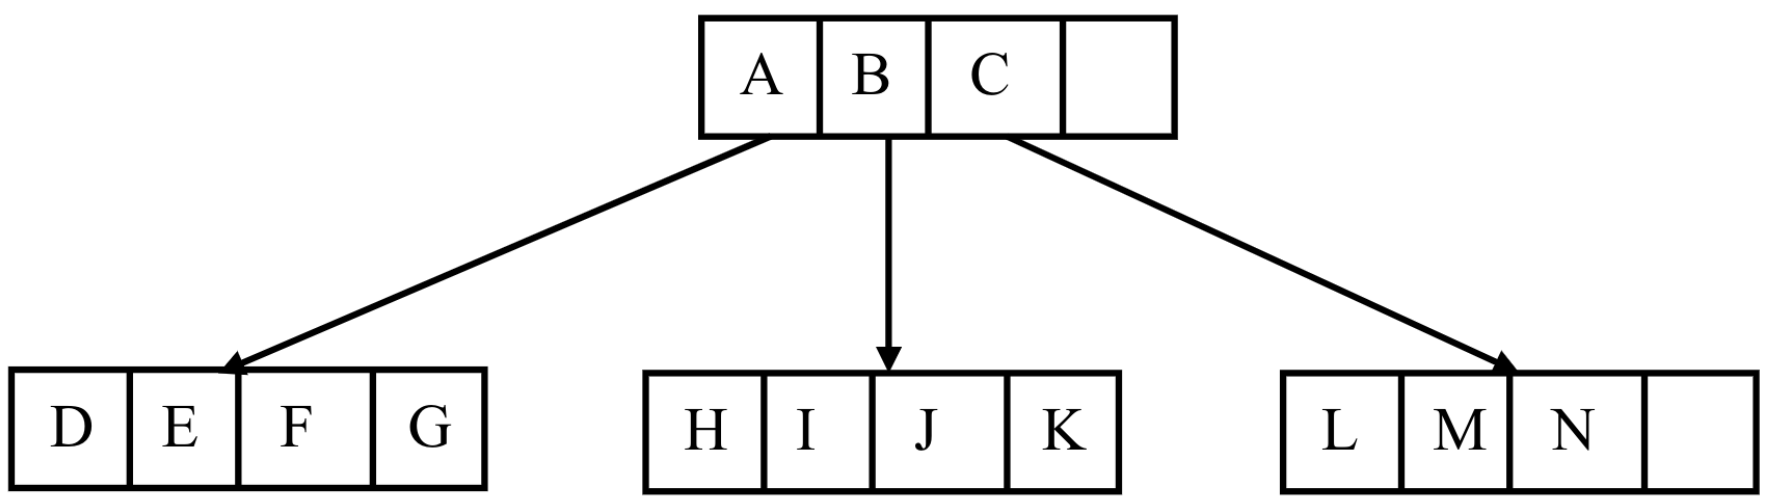
\includegraphics[width=\linewidth]{./figures/rtree.png}
    \caption{The corresponding R-tree, from \cite{rtree}.}
    \label{fig:rtree}
\end{figure}

What distinguishes a normal R-tree from a Hilbert R-tree is the MBR selection. The Hilbert R-tree utilizes Hilbert curves to generate MBRs for nodes. A Hilbert curve is a space-filling curve that can traverse every point in higher-dimensional space. This property allows for the mapping of two-dimensional values to one-dimensional values by drawing the curve in two dimensions and assigning ascending values to the points along the curve, see figure \ref{fig:hilbert} for Hilbert curves with corresponding values. These values are referred to as Hilbert values. Hilbert curves have the characteristic such that elements close in space will also be close in Hilbert values. By sorting MBRs based on the Hilbert value of the rectangle centroids, we can create MBRs with minimal overlap for spatial indexing.

\begin{figure}[t]
    \centering
    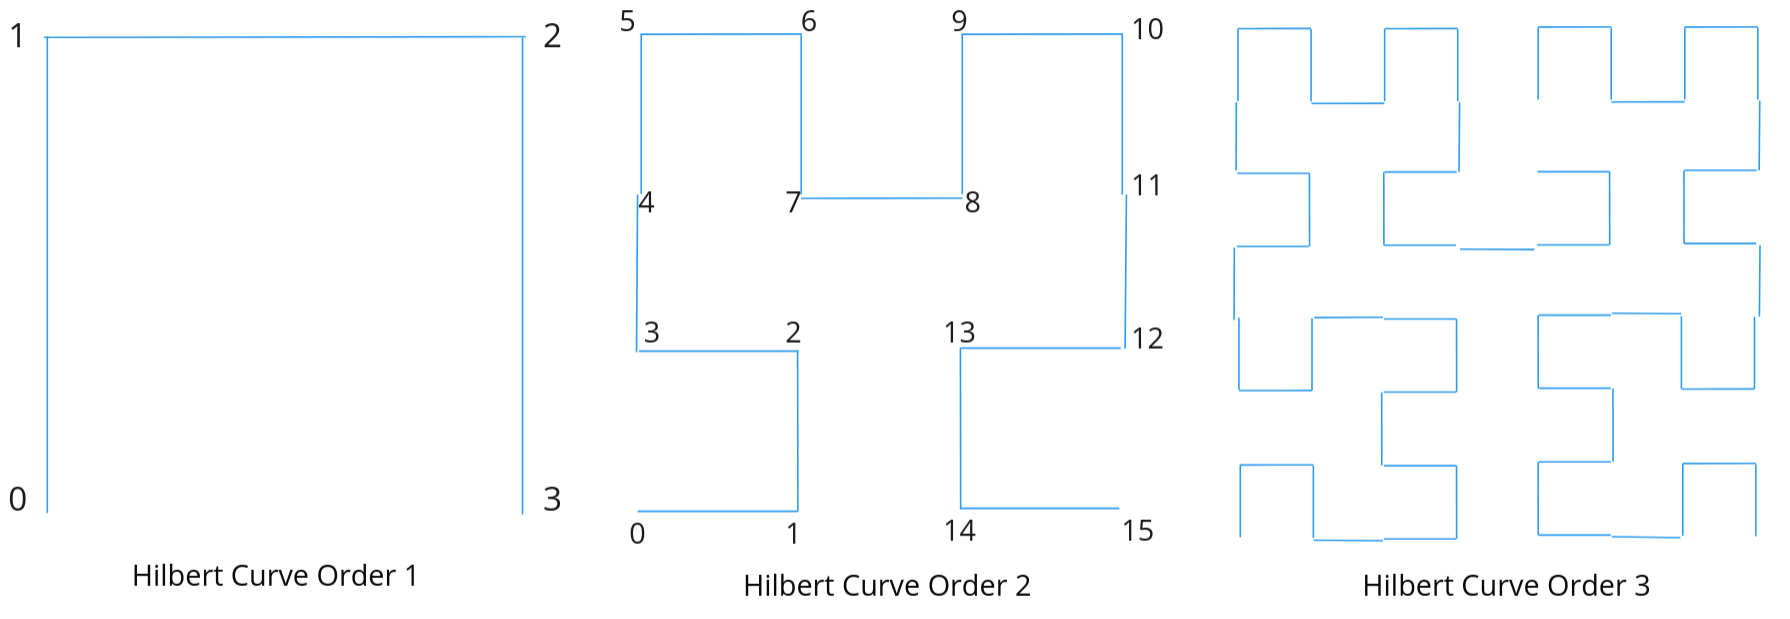
\includegraphics[width=\linewidth]{./figures/hilbert_orders.png}
    \caption{Showing Hilbert Curves of orders 1, 2, and 3.}
    \label{fig:hilbert}
\end{figure}

The Packed Hilbert R-tree is an optimized version of the Hilbert Tree. The Packed R-tree has even less overlap, resulting in improved query performance. The downside is that it requires more resources for construction. Considering the additional resource consumption, the Packed variant is only practical for applications that heavily prioritize read operations. In a system with frequent write operations, the entire tree would need to be rewritten frequently, leading to significant performance loss. For this reason, the Packed Hilbert R-tree is also known as the static Hilbert R-tree.